\documentclass[UTF8,10pt,a4paper]{ctexart}
\usepackage[margin=20mm,headheight=26pt]{geometry}
\usepackage{graphicx,xcolor,fancyhdr,booktabs,tabularx,enumitem,hyperref}
\definecolor{ink}{HTML}{12313B}\definecolor{teal}{HTML}{008F89}
\hypersetup{colorlinks=true,urlcolor=teal,linkcolor=teal,pdftitle={WorldGuard 提交材料}}
\setlength{\parindent}{0pt}\setlength{\parskip}{4pt}\linespread{1.12}
\setlist{nosep,leftmargin=1.5em}
\pagestyle{fancy}\fancyhf{}
\fancyhead[L]{\raisebox{-4pt}{
\includegraphics[height=8mm]{assets/logo.png}}\quad\textbf{\textcolor{ink}{WorldGuard}}}
\fancyhead[R]{\small 零界智行\quad U406}
\fancyfoot[L]{\footnotesize 本科生组 · 南京大学 / 东南大学}
\fancyfoot[R]{\footnotesize\thepage}
\renewcommand{\headrulewidth}{0.4pt}
\ctexset{section={format=\Large\bfseries\color{ink},beforeskip=12pt,afterskip=6pt},subsection={format=\large\bfseries\color{teal}}}
\newcommand{\cover}[2]{\vspace*{5mm}{\small\textcolor{teal}{WORLDGUARD / SUBMISSION 2026}}\par\vspace{4mm}{\huge\bfseries\color{ink}#1}\par\vspace{3mm}{\large #2}\par\vspace{4mm}\hrule\vspace{5mm}}
\newcommand{\note}[1]{\par\smallskip\noindent\colorbox{teal!7}{\parbox{0.95\linewidth}{\small #1}}\par\smallskip}
\begin{document}
\cover{公开项目记录与视频链接}{B站已发布页面核查 / 2026-10-15}
\textbf{平台：}哔哩哔哩\par
\textbf{标题：}WorldGuard｜基于 Agnes Harness 的移动机器人导航测试与验证工作台——零界智行 U406 项目演示\par
\textbf{有效链接：}\url{https://www.bilibili.com/video/BV1dQJ66tEsV/}\par
\textbf{页面显示发布时间：}2026-10-15 10:48:05\par
\textbf{播放器时长：}04:15。符合 3 至 5 分钟的时长要求。\par
\textbf{核查方式：}2026-10-15 在未登录状态打开该页面，看到视频播放、项目说明和发布日期。未使用参赛者个人账号。平台可能弹出可关闭的登录提示，提交前应再检查链接可用性。
\begin{center}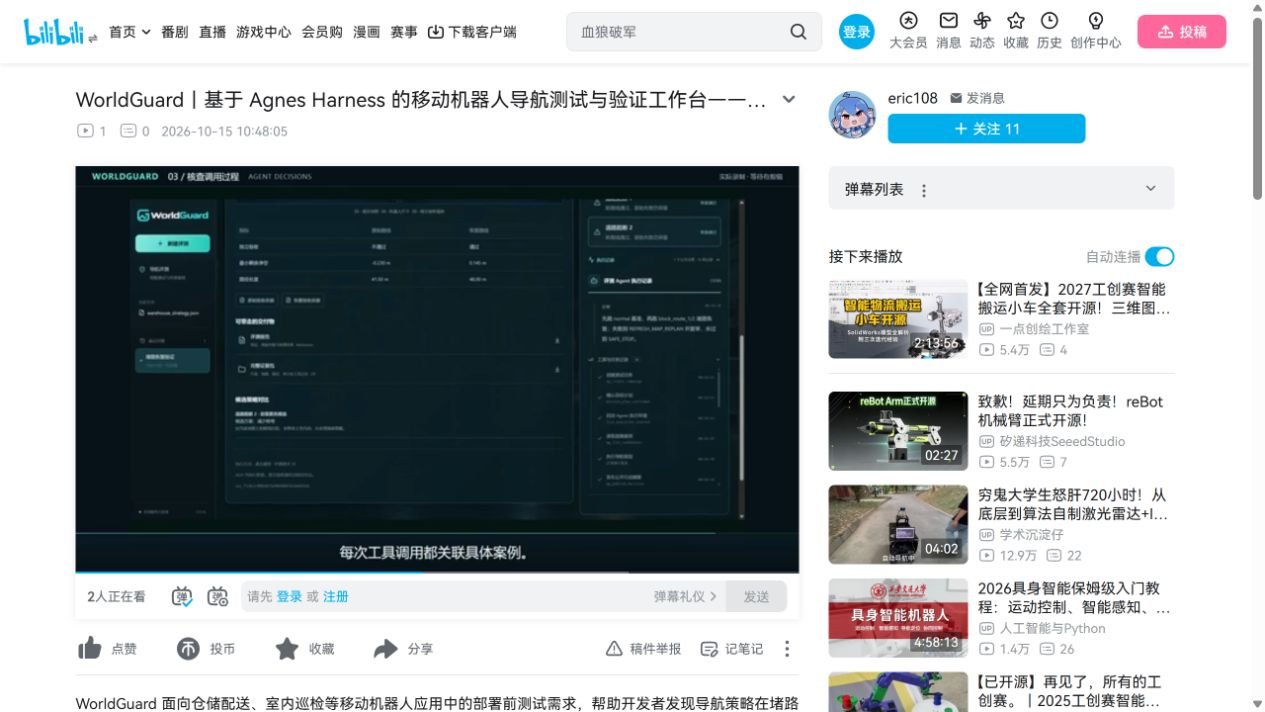
\includegraphics[width=\linewidth]{assets/bilibili-proof.jpg}\end{center}
以上为实际网页截图，未修改页面显示。另附用户提供的完整标题及日期截图。该链接同时作为演示视频主链接和至少一条公开真实项目记录；未提供备用视频链接。
\end{document}
